%%%%%%%%%%%%%%%%%%%%%%%%%%%%%%%%%%%%%%%%%
% Beamer Presentation
% LaTeX Template
% Version 1.0 (10/11/12)
%
% This template has been downloaded from:
% http://www.LaTeXTemplates.com
%
% License:
% CC BY-NC-SA 3.0 (http://creativecommons.org/licenses/by-nc-sa/3.0/)
%
%%%%%%%%%%%%%%%%%%%%%%%%%%%%%%%%%%%%%%%%%

%----------------------------------------------------------------------------------------
%	PACKAGES AND THEMES
%----------------------------------------------------------------------------------------

\documentclass{beamer}

\mode<presentation> {
	
	% The Beamer class comes with a number of default slide themes
	% which change the colors and layouts of slides. Below this is a list
	% of all the themes, uncomment each in turn to see what they look like.
	
	%\usetheme{default}
	%\usetheme{AnnArbor}
	%\usetheme{Antibes}
	%\usetheme{Bergen}
	%\usetheme{Berkeley}
	%\usetheme{Berlin}
	%\usetheme{Boadilla}
	%\usetheme{CambridgeUS}
	%\usetheme{Copenhagen}
	%\usetheme{Darmstadt}
	%\usetheme{Dresden}
	%\usetheme{Frankfurt}
	%\usetheme{Goettingen}
	%\usetheme{Hannover}
	%\usetheme{Ilmenau}
	%\usetheme{JuanLesPins}
	%\usetheme{Luebeck}
	\usetheme{Madrid}
	%\usetheme{Malmoe}
	%\usetheme{Marburg}
	%\usetheme{Montpellier}
	%\usetheme{PaloAlto}
	%\usetheme{Pittsburgh}
	%\usetheme{Rochester}
	%\usetheme{Singapore}
	%\usetheme{Szeged}
	%\usetheme{Warsaw}
	
	% As well as themes, the Beamer class has a number of color themes
	% for any slide theme. Uncomment each of these in turn to see how it
	% changes the colors of your current slide theme.
	
	%\usecolortheme{albatross}
	%\usecolortheme{beaver}
	%\usecolortheme{beetle}
	%\usecolortheme{crane}
	%\usecolortheme{dolphin}
	%\usecolortheme{dove}
	%\usecolortheme{fly}
	%\usecolortheme{lily}
	%\usecolortheme{orchid}
	%\usecolortheme{rose}
	%\usecolortheme{seagull}
	%\usecolortheme{seahorse}
	%\usecolortheme{whale}
	%\usecolortheme{wolverine}
	
	\setbeamertemplate{footline} % To remove the footer line in all slides uncomment this line
	%\setbeamertemplate{footline}[page number] % To replace the footer line in all slides with a simple slide count uncomment this line
	
	\setbeamertemplate{navigation symbols}{} % To remove the navigation symbols from the bottom of all slides uncomment this line
}

\usepackage{graphicx} % Allows including images
\usepackage{booktabs} % Allows the use of \toprule, \midrule and \bottomrule in tables

\usepackage{color}
\definecolor{red}{rgb}{1.0,0.,0.}
\newcommand{\todo}[1]{\textcolor{red}{[[#1]]}}
\usepackage{subfigure}

%----------------------------------------------------------------------------------------
%	TITLE PAGE
%----------------------------------------------------------------------------------------

\title[GPU polynomial computation]{Polynomial Computation on GPU} % The short title appears at the bottom of every slide, the full title is only on the title page

\author{Kevin Mueller} % Your name
\institute[UW] % Your institution as it will appear on the bottom of every slide, may be shorthand to save space
{
	\\ % Your institution for the title page
	\medskip
}
\date{\today} % Date, can be changed to a custom date

\begin{document}
	
	\begin{frame}
		\maketitle
	
		
	\end{frame}
	
	\section{Test section one}
	\begin{frame}
		\begin{center}
			\Huge Overview
		\end{center}
	
		\vspace{0.2in}
		Examples include:
		\begin{itemize}
			\item Symbolic Computing Basics (Polynomials)
			\item Motivating Examples
			\item GPU algorithms
			\item Project Outline
		\end{itemize}
		
	\end{frame}
	
	
	\begin{frame}
		\begin{center}
		\Huge Basics
		\end{center}
		\begin{align*}
		f(x) = \sum_{k=0}^{n} f_kx^k,\quad \text{with } f_n \ne 0 \space \text{ and } f_k \in \mathbb{D}
		\end{align*}
		
		\begin{itemize}
			\item $f_kx^k$ is a monomial of f.
			\item The degree $\deg(f)$ of f is the largest integer such that $f_n \ne 0$.
			\item zero polynomial (i.e $f_k = 0 \text{, } \forall \text{ }k$), $\deg(0) = -\infty$
			\item $f_n$ is called leading coefficient $\text{lcf}(f)$
			\item Smallest integer $l$ for $f_l \neq 0$ is the trailing coefficient.
			\item A polynomial is monic of its leading coefficient equals $1$.
		\end{itemize} 
		
	\end{frame}
	
	\begin{frame}
		
		
		A Unique Factorization Domain (UFD) is an integral domain with the additional property that any non-zero $a \in D$ is either unit or can  be expressed as a finite product of irreducible elements $a = p_1p_2\dots p_n$.	
		
		\vspace{0.2in}
		
		This implies that the $\gcd(a,b)$ always exists.
		\vspace{0.2in}
		
		Integers $\mathbb{Z}$ are a UFD whose only units are $1$ and $-1$.
		\vspace{0.2in}
		
		Closely related is the concept of relatively prime. For any two elements $a,b \in \mathbb{D}$, $\gcd(a,b) = 1$.
					
	\end{frame}
	
	\begin{frame}
		
			\begin{figure}[!ht]
				\centering
				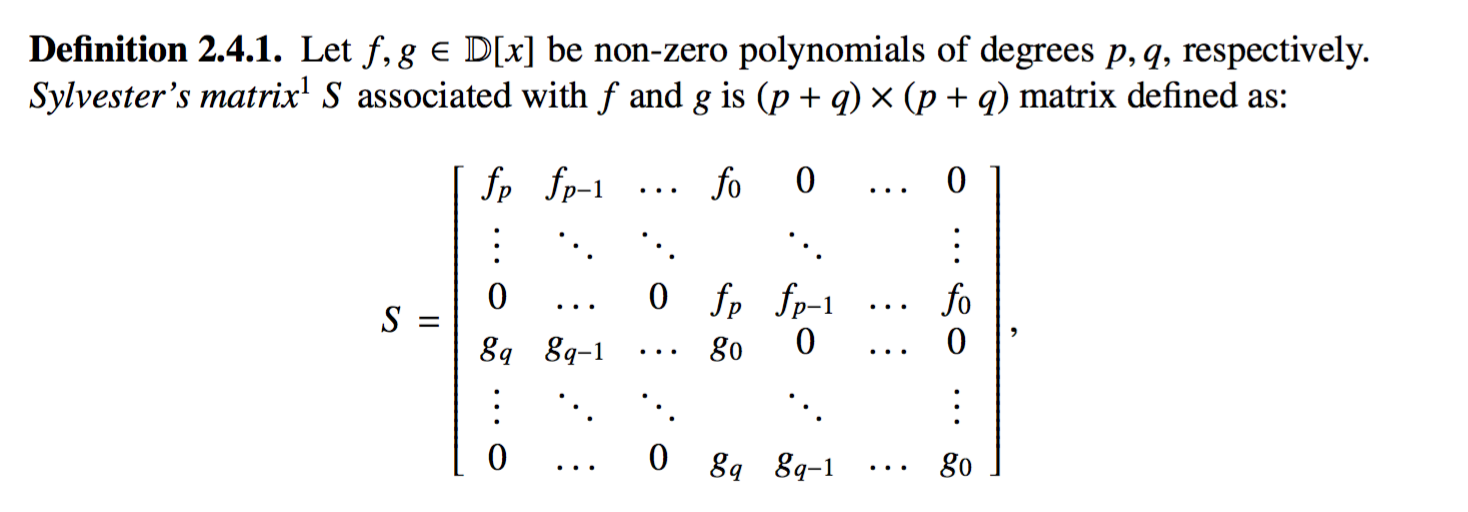
\includegraphics[width=0.925\textwidth]{../Code/Images/sylv_matrix.png}
			\end{figure}
			
		
		In general we can reduce our symbolic polynomial computations to computing greatest common denominators (GCDs),resultants and subresultants.
		\vspace{0.2in}
		
		The resultant is an elimination tool that gives an algebraic formulation to decide whether a system of polynomial equations has a common solution expressed in terms of their coefficients.
		\vspace{0.2in}
			
		Subresultants relate the GCD of two polynomials and their resultants by looking at a submatrix of the Sylvester matrix.
		
		\vspace{0.2in}
		
	
		
		
		
		
	\end{frame}
	
	\begin{frame}
		\begin{center}
			\Huge Motivating Example
		\end{center}
		
		Let's attempt to compute the intersection of two algebraic surfaces of degree 4.
		
		\begin{align*}
			(10y^2 + z^2 - 112)^2 - 5z^4y^4 + xy^4 - 1 = 0 \\
			50(x^2y^2 + y^2z^2 + x^2z^2) + (x^2 + y^2 + z^2 -1)^2 = 0
		\end{align*}
	
	
		
	\end{frame}
	
	\begin{frame}
		
		The intersection is given by an algebraic curve in 3D which when projected onto the x-y plane satisfies the equation:
		
		\begin{figure}[!ht]
			\centering
			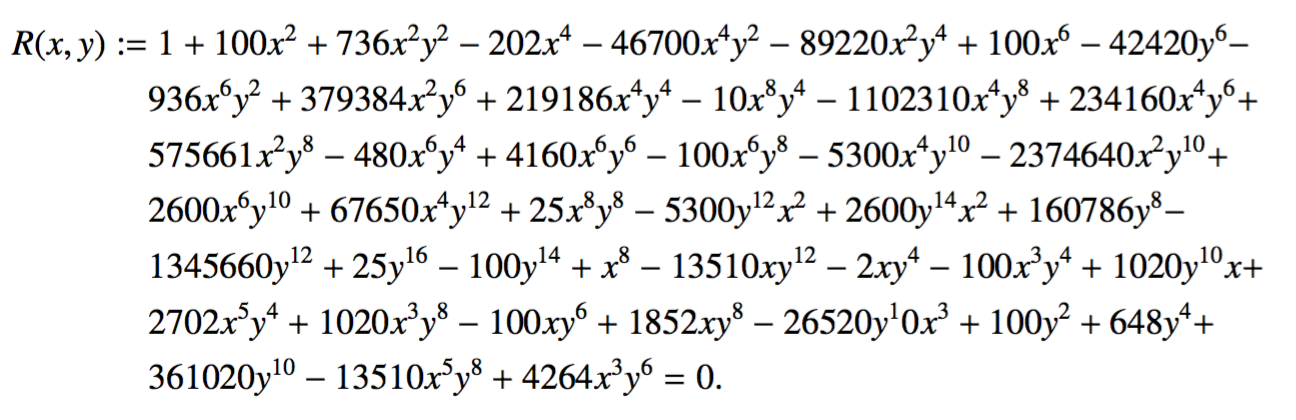
\includegraphics[width=0.825\textwidth]{../Code/Images/R_xy_proj.png}
			\label{fig:FF_book_image}
		\end{figure}
		
		Analyzing the topological structure of $R(x,y)$ involves computing the resultant of $R$ and $R'y$, which becomes a dense polynomial of 132 degrees and $500$ coefficients.
		\vspace{0.2in}
		
		Increasing the degree slightly, creates a polynomial of degree $2028$ and $4500$ coefficients.
		
		 
	\end{frame}
	
	\begin{frame}
		For a more concrete example, consider the skeleton/medial axis computation in 2D. As we know points on the skeleton/medial axis correspond to singular points of the signed distance function. However the SDF is generally not available, so computing the gradient components and setting them to zero is not possible.
		
		\vspace{0.2in}
		Geometric Viewpoint:
		\begin{itemize}
			\item The closest surface point
			\item the largest circle contained within the closure of the object makes contact with the surface.
			\item The maximal circle has at least 2 distinct points of 2nd order contact, when ignoring circles that contact the boundary at a singular point.

		\end{itemize}		
		
				
		
	\end{frame}
	
	\begin{frame}
		Let $f(x,y,z)$ be the polynomial function that implicitly defines the object.
		
		Let $g$ be the implicit definition of a circle given by,
		$$g(x,y,z,x_0,y_0,z_0,r) = (x-x_0)^2 + (y-y_0)^2 + (z-z_0)^2 - r^2$$
		
		There must be 2 contact points that lie on the surface of the object:
		$f_1 = f(x_1,y_1,z_1) $ and $f_2 = f(x_2,y_2,z_2) = 0$
		
		$$h1 = \nabla f_1 \times \nabla g_1 = 0 $$
		$$h2 = \nabla f_2 \times \nabla g_2 = 0 $$
		
		Distinct Criterion: $k\left\{(x-x_0)^2 + (y-y_0)^2 + (z-z_0)^2\right\} - 1$		
		
		
	\end{frame}
	
	
	\begin{frame}
		
		\begin{figure}
			\centering
			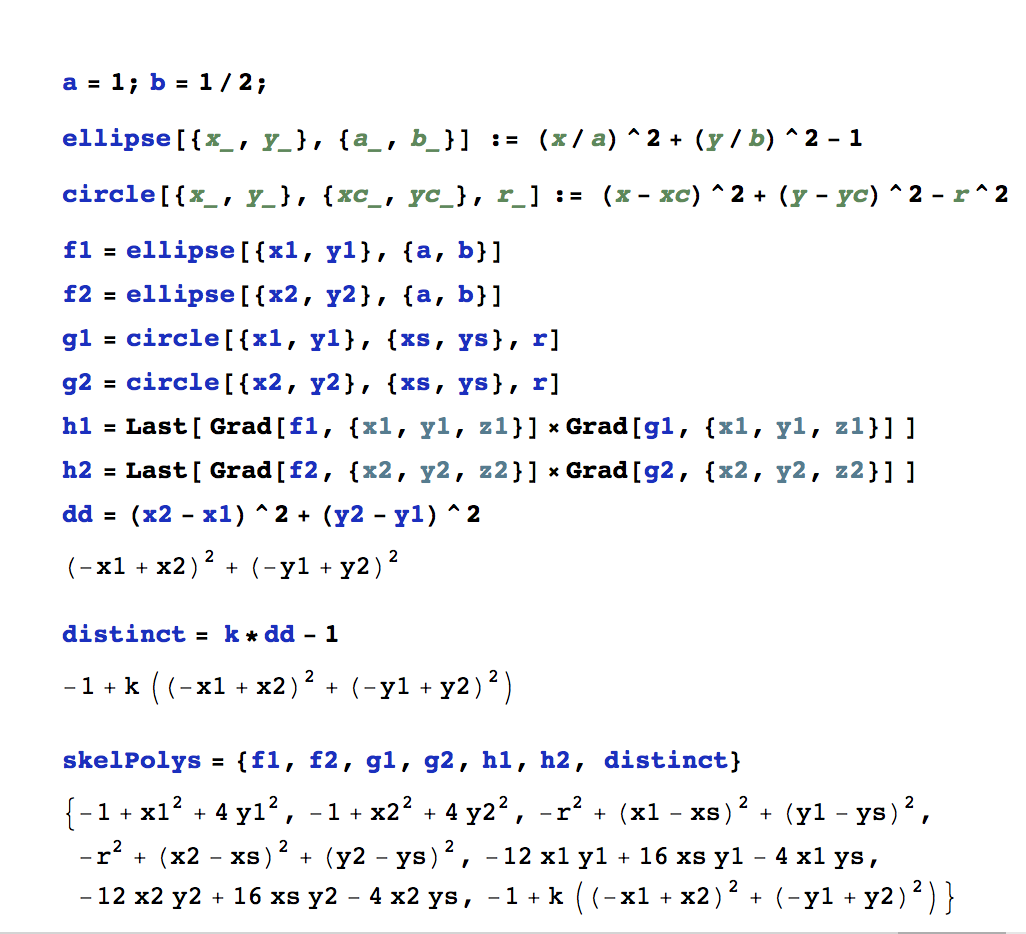
\includegraphics[width=0.825\textwidth]{../Code/Images/code_skeleton.png}
		\end{figure}
		
	\end{frame}
	
	\begin{frame}
		\begin{figure}
			\centering
			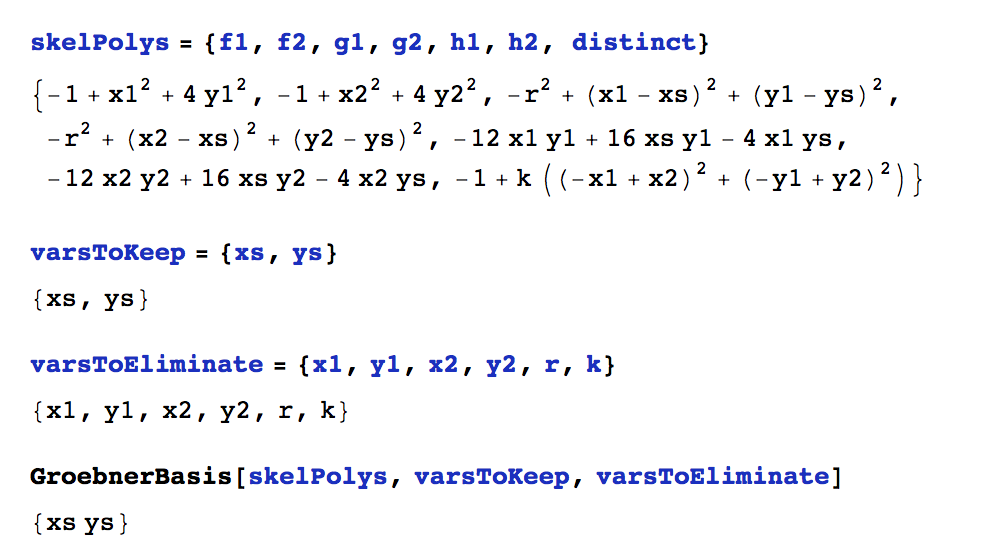
\includegraphics[width=0.825\textwidth]{../Code/Images/code_skeleton_3.png}
		\end{figure}
		
		\vspace{0.2 in}
		
		The important part for the polynomial computation is the "GroebnerBasis" Line.

	\end{frame}
	
	
	\begin{frame}
		\centering
		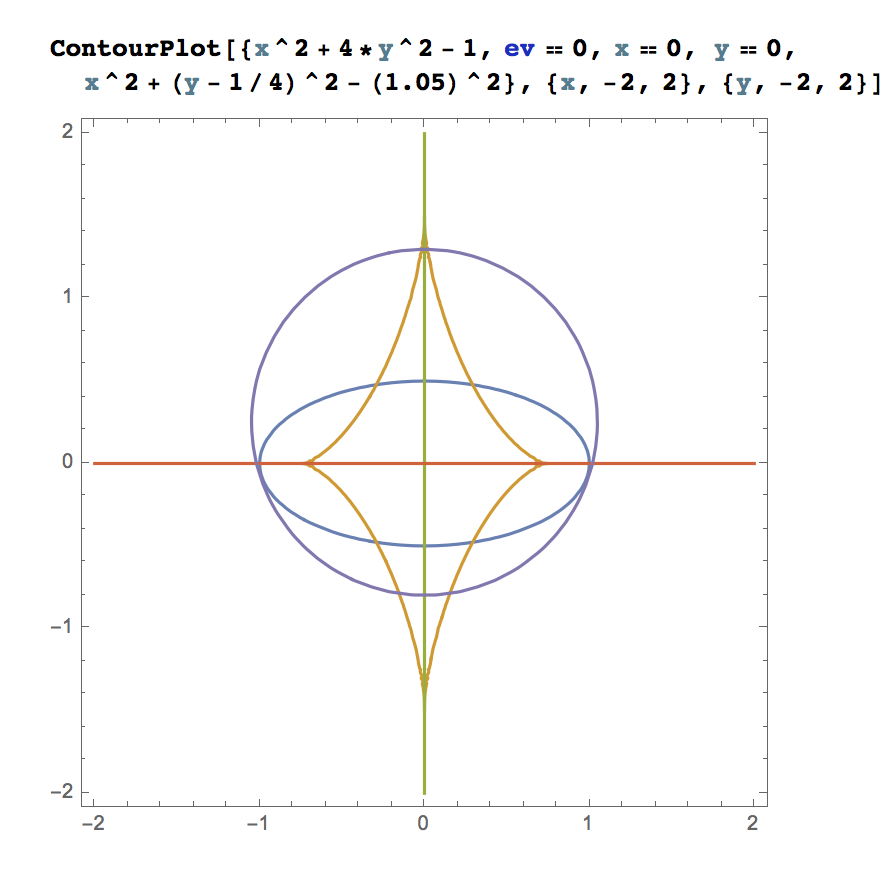
\includegraphics[width=0.825\textwidth]{../Code/Images/Ellipse_structure.png}
	\end{frame}
	
	\begin{frame}
		\begin{center}
			\Huge GPU Algorithms
		\end{center}
		\begin{itemize}
			\item Employ a divide and conquer strategy (Homomorphisms)
			\item Chinese Remaindering
			\item Polynomial interpolation
		\end{itemize}
	\end{frame}
	
	
	\begin{frame}
		\centering
		\vspace{0.4in}
		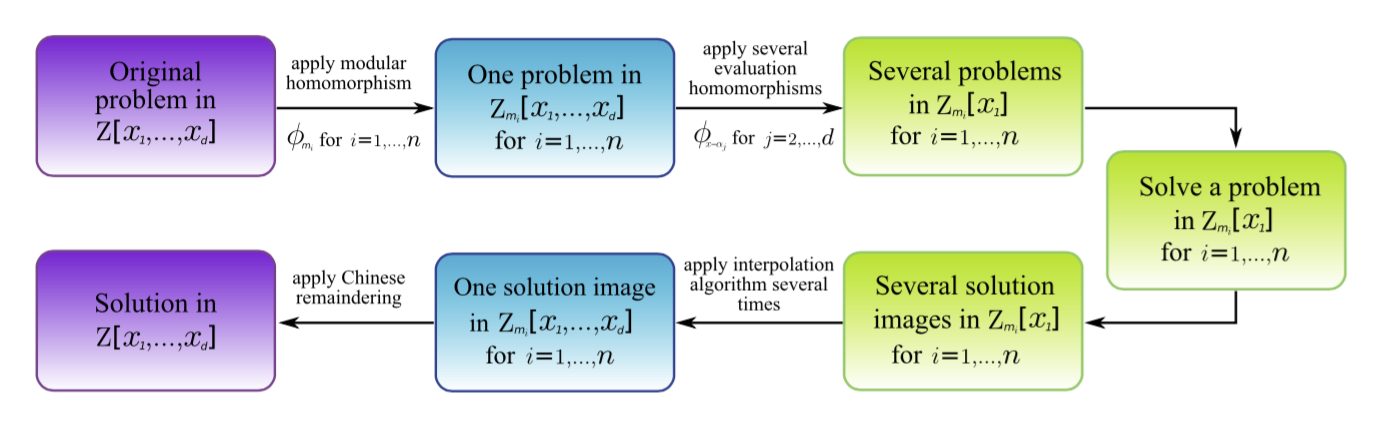
\includegraphics[width=0.995\textwidth]{../Code/Images/diagram_homomorphisms.png}
	\end{frame}
	
	

	\begin{frame}
		\begin{center}
			\huge Project Outline
		\end{center}
		
		\begin{itemize}
			\item Implement the above scheme using CUDA
			\item Attempt to specialize and apply it to a particular application such as solid sweeping or Medial/Skeleton computations.
			\item Compare the results.
			\item Look at other interpolation strategies such as Chebychev polynomials. 
			\item Other extensions?
			
		\end{itemize}
		
	\end{frame}
	
	
	
	
	%------------------------------------------------
	
	\begin{frame}
		\frametitle{References}
		\footnotesize{
			\begin{thebibliography}{99} % Beamer does not support BibTeX so references must be inserted manually as below
				\bibitem[FF]{p1} Duane Storti 
				\newblock appliedPolynomialComputation
				
				\bibitem[GW]{p1} Pavel Emeliyanenko
				\newblock Harnessing the Power of GPUs for Problems in Real Algebraic Geometry.
				\newblock \emph{PhD thesis, Universität des Saarlandes, 2012} 
			\end{thebibliography}
		}
	\end{frame}
	
\end{document} 